\section{Introdução} \label{sec:intro}

% 1. Introdução
%    1. Motivação
%       1. entre as duas conectar c como e pq simular
%    2. Lacunas (Revisão Bibliográfica, estado da arte)
%    3. Justificativa
%    4. Objetivos (e Hipótese)
%    5. Contribuição Científica

% Importância de trabalhar com combustão no contexto global.
% Como se simula combustão
% Necessidade de modelos HMT para partículas em simulações de combustão e sua importância

% Explain need for multicomponent modeling in current global context
% Explain need for modeling the interior of the droplet
% Explain need for droplet combustion model

% GAP: lack of models for single droplet combustion, modeling way behind pure evaporation
% GAP: lack of consistent multicomponent version of evaporation models and lack of multicomponent single-droplet burning models.
% GAP: lack of computationally affordable methods that account for droplet interior AND advanced evaporation/SDC models.

A demanda pela transição energética e pela descarbonização da economia busca alternativas para substituição dos combustíveis fósseis nos setores de energia, transporte, indústria. 
Alguns setores, como o energético e o de transportes urbano de baixa carga, têm mostrado grande progresso no uso de energias renováveis e na eletrificação, respectivamente \cite{MasriA2021}. 
Porém, combustíveis fósseis são extremamente difíceis de substituir em outros setores, especialmente os combustíveis líquidos.
Estes possuem maior energia específica e densidade energética \cite{Bergthorson2017,Julien2017}, assim adequados para aplicações de transporte, como no setor automotivo de cargas pesadas, naval e aeronáutico \cite{MasriA2021}.
Combustíveis líquidos são importantes também para algumas indústrias como aço e cimento, para algumas termoelétricas e até para máquinas de pequeno porte portáteis movidas a motor de combustão interna (MCI).
Soma-se a isso uma análise histórica que indica que a transição para fontes renováveis se dará ao longo de décadas \cite{MasriA2021}.

% #TODO 4 O etanol, em particular, é de grande relevância para o Brasil e para a India. 

Nota-se que processos de combustão continuarão relevantes nas próximas décadas.
Em especial, todas as aplicações mencionadas baseiam-se na combustão turbulenta de sprays líquidos.
Assim, soluções devem ser procuradas para conciliar essa tecnologia com os esforços de transição energética e descarbonização da economia.
A comunidade científica busca, então, três caminhos: \textbf{(i)} desenvolver tecnologias para novos combustíveis (como  etanol, metanol, hidrogênio e amônia \cite{FAPESP_etanol_1,VerhelstS2019,TeohY2023,ElbazA2022}); \textbf{(ii)} desenvolver novas origens para os mesmos combustíveis (como SAF, biocombustíveis e eletro-combustíveis \cite{BenJames-SAF,BergthorsonJ2015,WestbrookC2019,PalysM2022}); \textbf{(iii)} melhorar a eficiência dos motores a combustão e reduzir a formação de poluentes \cite{MasriA2021}.

Independente da origem do combustível, o processo de combustão deve ser compreendido para que motores e queimadores eficientes e com baixa emissão de poluentes sejam desenvolvidos.
Para tanto é necessário pesquisa em combustão, que pode ser estruturada em trabalhos experimentais e trabalhos de modelagem.
A modelagem da combustão turbulenta de sprays, foco dessa proposta, deve ser capaz de contemplar diferentes combustíveis líquidos, incluindo combustíveis oriundos das demandas (i) e (ii).
Deve também representar os diferentes fenômenos envolvidos nesse processo, como ignição e formação de poluentes, para atender a demanda (iii).
No âmbito da combustão turbulenta de sprays, é de extrema importância o modelo de transferência de calor e massa da gota (líquida) para a fase gasosa (HMT -\emph{Heat and Mass Transfer}).
Modelos HMT regem, dentre outros aspectos, a taxa de vaporização do combustível das gotas do spray.
É conhecido que essa modelagem tem enorme influência na chama \cite{JennyB2012}, influenciando a sua estrutura, temperatura, geometria e formação de poluentes.


Nesse sentido, revisando a literatura mais recente, nota-se a necessidade de maior desenvolvimento de \textbf{modelos de evaporação e condensação} (MEC) para representar corretamente diferentes combustíveis.
Por exemplo, modelos monocomponentes com equilíbrio termodinâmico não são capazes de representar todos os fenômenos associados, por exemplo, à combustão de etanol \cite{SacomanoF2024CF}, combustível de importância estratégica para o Brasil e para a Índia \cite{etanol-BNDES,etanol-India}.
Em especial, nota-se uma demanda pela aplicação de modelos sofisticados, desenvolvidos e testados na escala de uma única gota ou em simulações
laminares ou unidimensionais, em simulações multidimensionais de combustão turbulenta.
Para representar combustíveis reais como o etanol é necessário modelar a gota com abordagem de substância \textbf{multicomponente}, considerando \textbf{termodinâmica de mistura não-ideal} e os efeitos de transferência de calor e massa no \textbf{interior da gota}.

% No modelo descrito acima, a reação química é resolvida separadamente do modelo da gota. 
% Isso corresponde a uma chama longe e não presa a gota, em que a chama é alimentada pelo vapor de combustível oriundo de várias gotas evaporando.
% Em contraste, é possível que ocorra a combustão de uma gota isolada, com uma frente de chama próxima e circundante à gota, a uma distância na mesma ordem de grandeza que o diâmetro da gota.
Em MECs, a evaporação da gota fornece vapor de combustível que alimenta a chama.
Nessa abordagem, a chama não é estabilizada por uma gota em específica, mas se estabilizada por fenômenos específicos ao escoamento gasoso \cite{ChiuH1982,Law2006}.
Esse modo de combustão de spray é chamado \textbf{combustão com frente de chama externa}, ou simplesmente \textbf{combustão externa}.
Em contraste, é possível que as gotas entrem em combustão individualmente, com a evaporação de combustível alimentando uma frente de chama próxima e envolvente a cada gota, a uma distância na mesma ordem de grandeza que o diâmetro da gota \cite{ChiuH1977}.
Isso é chamado \textbf{combustão de gota isolada}.

Experimentos indicam que a combustão de gota isolada ocorre tanto durante a ignição	de sprays \cite{AggarwalS2014} quanto em sprays já desenvolvidos \cite{ChenG1996CF,SinghG2020,GounderJ2009PhD}.
Simulações DNS (\emph{Direct Numerical Simulation}) e LES (\emph{Large Eddy Simulation}) também indicam a ocorrência de combustão de gota isolada nessas duas etapas da combustão turbulentas de sprays líquidos (\cite{BorghesiG2013CF} e \cite{PaulhiacD2020,BojkoDesJardin2017CF}, respectivamente).
A combustão de gota isolada também ocorre na combustão de alguns pós metálicos que queimam em combustão homogênea na fase gasosa, como o alumínio \cite{Bergthorson2015,Julien2017,Baumann2020}, segundo várias evidências experimentais \cite{Braconnier2020Pre,Braconnier2022,Bucher1999,Halter2023}.
A Figura \ref{fig:sdc-exp} mostra evidências da combustão de gota isolada em sprays turbulentos de etanol (Figuras \ref{fig:GounderJ2009-7.17} e \ref{fig:SinghG2020-10}) e na combustão de uma partícula alumínio (Figura \ref{fig:Braconnier202PhD-5.20}). %\todo{explicar figuras ...}

Além disso, alguns trabalhos apontam para a combustão de gota isolada em sprays líquidos como uma fonte de emissão de fuligem \cite[e referências 3-13 \emph{loc. cit.}]{FachiniF2005}, de forma que a modelagem desse fenômeno contribui com os esforços de limitar as emissões desse poluente.

% A Fig. \ref{fig:GounderJ2009-7.17}, adaptada de \cite{GounderJ2009PhD}, mostra a chama EtF4 do queimador experimental de Sydney \source{} usando LIF-OH (\emph{Laser Induced Fluorescence} do radical OH), 

\begin{figure}[H]
    \centering
    \caption{Observações experimentais de combustão de gota isolada em chamas de etanol na Fig. \ref{fig:GounderJ2009-7.17} e \ref{fig:SinghG2020-10}, indicadas por setas, e ao redor de uma partícula de pó de alumínio na Fig. \ref{fig:Braconnier202PhD-5.20}. 
    Siglas: LIF -- \emph{Laser Induced Fluorescence}; HR -- \emph{Heat Release}.
    Adaptadas de \cite{GounderJ2009PhD,SinghG2020,Braconnier2020Pre}.
    }
    \begin{subfigure}[t]{0.39\textwidth}
        \centering
        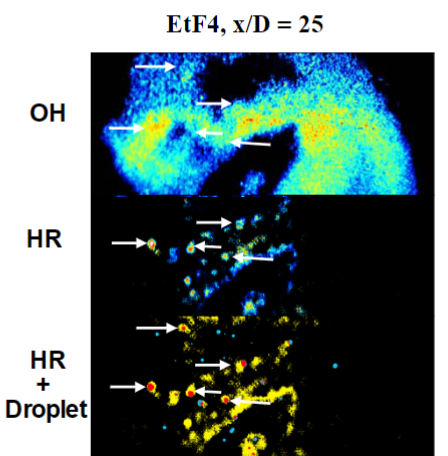
\includegraphics[width=0.99\textwidth]{30_images/GounderJ2009-7.17-1.png}
        \caption{LIF de OH, HR e HR sobreposto com posição das gotas em uma chama de etanol no queimador \emph{Sydney piloted spray burner}, 25 diâmetros do injetor a jusante. Adaptado de \cite[Fig. 7.13]{GounderJ2009PhD}.}
        \label{fig:GounderJ2009-7.17}
    \end{subfigure}
    \hfill
    \begin{subfigure}[t]{0.59\textwidth}
        \centering
        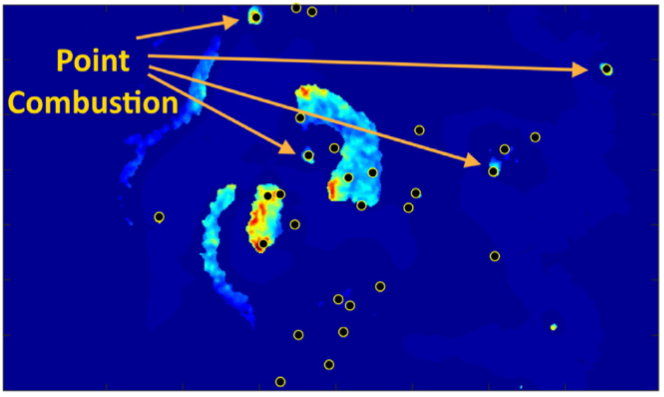
\includegraphics[width=0.99\textwidth]{30_images/SinghG2020-10.png}
        \vfill
        \caption{HR sobreposto com posição das gotas em uma chama de etanol no queimador \emph{Sydney piloted needle spray burner}, 20 diâmetros do injetor a jusante. Adaptado de \cite[Fig. 10]{SinghG2020}.}
        \label{fig:SinghG2020-10}
    \end{subfigure}
    \vspace{0.5cm}
    \begin{subfigure}[b]{0.8\textwidth}
        \centering
        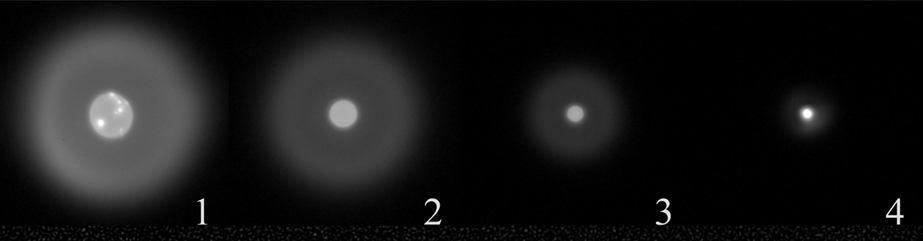
\includegraphics[width=0.99\textwidth]{30_images/Braconnier202PhD-5.20.png}
        \caption{Fotografias de combustão de uma partícula de alumínio de $\qntdd{50}{\mu m}$ de diâmetro em atmosfera 80\% Argônio/ 20\% oxigênio. Adaptado de \cite[Fig. 5.21]{Braconnier2022}.}
        \label{fig:Braconnier202PhD-5.20}
    \end{subfigure}
    \label{fig:sdc-exp}
\end{figure}

% A combustão de gota isolada é uma etapa essencial para a ignição de sprays, como discutido pela revisão \cite{AggarwalS2014} e observado, por exemplo, em \cite{BorghesiG2013CF}. 
% Além disso, estudos indicam que a combustão de gota isolada está relacionada a emissão de carbono particulado \cite{FachiniF2005}, 
% Dessa forma, modelar a combustão de gota 

Assim, constata-se que modelar a combustão de gota isolada é importante para a ignição de sprays de combustíveis líquidos, para a emissão de poluentes (em particular de fuligem) e também para a combustão de alguns combustíveis metálicos. 
Revisando a literatura, constatou-se a necessidade de desenvolver modelos de combustão de gota isolada (MCGI) capazes de representar corretamente diferentes combustíveis, incluindo as mesmas capacidades mencionadas para os MECs.
Notou-se também que não é claro na literatura quando a combustão de gota isolada ocorre \cite[p. 8]{JennyB2012} -- apesar de existirem diferentes modelos em cenários simplificados, a serem discutidos -- nem a influência de modelar a combustão de gota isolada (MCGIs) junto com a combustão externa (representada por MECs) na combustão turbulenta multidimensional.
% \todo{Mencionar aumento na complexidade teórica do modelo HMT.}
% nem o seu efeito na combustão turbulenta multidimensional.
% Diferentes modelos existem para determinar quando ocorre a combustão de gota isolada, como o modelos de Chiu \cite{ChiuH1977}, o de Borghi \source{Borghi1996}, o de Reveillon e Vervisch \source{Reveillon2005} e o Franzelli \source{FranzelliB2016CF}, porém nenhum é amplamente utilizável.
% Sabe-se que a combustão de gota isolada é importante para a ignição do spray \cite{AggarwalS2014}, mas não foram encontrados estudos sobre o seu impacto na estrutura da chama.
% Notou-se também a
% Mencionar objetivo ser o desenvolvimento de modelos robustos e eficientes para aplicação em CFD.  #DONE


\subsection{Objetivos} \label{sec:objetivos}

Tendo em vista os aspectos levantado anteriormente, a tese proposta tem como objetivo o \orange{desenvolvimento de estratégias para a simulação da transferência de calor e massa} em gotas em dois cenários: (\textbf{A.}) combustão externa; (\textbf{B}.) combustão de gota isolada.
Esses cenários correspondem aos seguintes modelos HMT:
\begin{enumerate}
    \item[\textbf{A.}] Modelo de Evaporação e Condensação (MEC); e 
    \item[\textbf{B.}] Modelo de Combustão de Gota Isolada (MCDI).
\end{enumerate}
Esses modelos devem considerar os seguintes aspectos: 
\begin{enumerate}
    \item[\textbf{1.}] Descrição multicomponente da gota; 
    \item[\textbf{2.}] Gota com termodinâmica de mistura não-ideal; 
    \item[\textbf{3.}] Consideração dos feitos de transferência	de calor e massa no interior da gota. 
\end{enumerate}
O objetivo é desenvolver aplicar a estratégia desenvolvida em simulações turbulentas reativas multidimensionais, com ambos modelos, {A} e {B} e com a funcionalidade:
\begin{enumerate}
    \item[\textbf{4.}] Determinação de quando ocorre a combustão de gota isolada;
\end{enumerate}
ou seja, de determinar se a gota se encontra no cenário {A} ou {B} e escolher o modelo apropriado para a correta representação dos fenômenos envolvidos.
Visando a aplicação em simulações CFD (\emph{Computational Fluid Dynamics}) turbulentas, reativas e multidimensionais, as estratégias a serem desenvolvidas devem ser robustos e computacionalmente eficientes.

O modelo HMT de simulações CFD que utilizem as estratégias a serem desenvolvidas, que incluem as funcionalidades {1}, {2} e {3}, e que possua a funcionalidade {4}, terá maior complexidade teórica em comparação aos modelos utilizados pela literatura. 
Isso permitirá ao autor dessa proposta investigar o efeito de considerar a combustão de gota isolada, e dos aspectos {1}, {2} e {3}, na estrutura da chama.
A investigação da estrutura da chama inclui a investigação de aspectos como distribuição de temperatura e concentrações de espécies, o que é essencial para a determinação da ignição, da eficiência de combustão e das emissões de poluentes.
A relação da estratégia a ser desenvolvida com a emissão de poluentes e com a ignição de sprays também será investigada. \question{Que tal? Deixei vago de propósito.}
% O papel dos efeitos das estratégias a serem desenvolvidas na emissão de poluentes e de  
% \question{Eu mencionei 3 motivos para estudar MCGI na pág anterior. E meu objetivo principal não é nenhum deles. Será que eu incluo os motivos um e dois como objetivos também?}


% A modelagem de combustão de gota isolada (MCGI), reduz a complexidade do problema de cinética química da simulação, mas aumenta a complexidade do modelo de transferência de calor e massa da gota, quando comparado ao modelo de evaporação/condensação (MEC).
% Assim, faz sentido desenvolver MEC primeiro, e depois o MCGI.
% Também, considerando que o objetivo é realizar uma simulação de chama turbulenta que use tanto um MEC quanto de um MCGI, é desejável que ambos tenhas as mesmas capacidades, (1) a (3).
% Por esse motivo, e considerando que, para simular, uma chama turbulenta de spray é necessário tanto um MEC quanto um MCGI,

% Utilizando essa abordagem, obtém-se, em larga escala, chamas ao redor de um grupo de gotas, internas ou exernas ao grupo (\emph{internal group combustion} ou \emph{external group combustion}), ou frentes de chama externas e não envovlventes (\emph{external sheath combustion}).
% Porém, uma frente chama também pode se formar ao redor de uma única gota, condição chamada combustão de gota isolada (\emph{single droplet combustion}).
% Revisando literatura, nota-se que não é claro quando a combustão de spray ocorre em cada modo \source



% São escoamentos particulados, dispersos e reativos, que envolvem fenômenos multi-escala, multifásicos e, frequentemente, combustíveis multicomponente.
% Revisando a literatura mais recente, o autor notou a ausência de estudos investigando a influência de modelar a combustão de gota isolada na estrutura da chama.
% Ademais, há um atraso em termos de complexidade na utilização de modelos de transferência de massa e calor (HMT - \emph{heat and mass transder}) em gotas nas simulações de larga escala, em comparação com simulações de uma única gota.
% Revisando a literatura mais recente, constatou-se uma dificuldade de identificar e modelar diferentes modos de combustão de spray.
% \colorbox{cyan}{Em particular, como a combustão isolada de gotículas afeta a estrutura da chama.}

% Na área da modelagem, que é foco dessa pesquisa
% Como se entende o processo ... experimento e modelagem ... foco em modelagem e simulação ... CFD.
% A simulação de combustão gasosa já é bem complexa, em parte devido à coexistência de fenômenos químicos e fenômenos de transporte, assim pela influência da turbulência e as interações entre esses aspectos.
% A combustão de sprays traz a complexidade adicional de possuir duas fases: uma fase contínua e gasosa, e uma fase dispersa, geralmente líquida.
% Escoamentos bifásicos como no caso de aerosóis ou sprays já são bem complexos, mesmo quando não reativos.
% Talvez por isso, para a simulação de escoamentos reativos de sprays, para parte química, utiliza-se técnicas desenvolvidas para a combustão gasosa.
% Combustíveis ... a maioria é líquido ... maior complexidade e desafios ...
% Foco em combustão de sprays líquidos ... 

% A modelagem para a sinulação de escoamentos reativos, dispersos e multifásicos, como na combustão de sprays, requer três partes: (i) a modelagem da fase contínua gasosa; (ii) a modelagem da fase dispersa, líquida; (iii) a modelagem da química homogênea, i.e. da combustão na fase gasosa.
% Para a parte (iii), a maioria dos trabalhos de combustão de sprays utiliza metodologias desenvolvidas para a combustão gasosa, considerando as gotas apenas como fontes de vapor de combustível.
% Isso corresponde 

% Necessidade e dificuldade de simular a combustão turbulenta de Sprays... Mencionar revisões ... que tipos de simulação tem .. dificuldade e necessidade de simulações de larga escala ... normalmente com química tabelada.

% Âmbito e objetivo desse trabalho.

% Necessidade e dificuldade de representação multicomponente da gota.

% Necessidade e dificuldade de representar o interior da gota.

% Necessidade e dificuldade de representar diferentes modos de combustão de gota -> combustão de gota isolada.

% No cenario atual de busca pela transição energética e descarbonização, a pesquisa em combustão é mais importânte do que nunca.
% Nesse contexto, os principais objetivos são reduzir emissões, adaptar os modelos para novos combustíveis mais limpos e para novos modos de combustão, necessários para motores mais limpos.

% Análises históricas indicam que a transição para fontes de energia renováveis se dará ao longo de décadas \cite{MasriA2021}, [MASRI 1, 3 também]. Até lá, combustíveis fosseis mantém o seu domínio.
% Além disso, no setor de transportes, a eletrificação dificilmente substituirá combustíveis fósseis em veículos de cargas pesadas ou para transporte aéreo ou marítmo, mesmo considerando previsões otimistas para o desevolvimento de baterias \cite{MasriA2021}. O mesmo pode ser dito para processos industriais intensivos em energia, como cimento e aço.

% Enquanto os caminhos (i) e (ii) concerne principalmente, aos químicos, o caminho (iii) requer a modelagem de processos de combustão. 
% A primeria abordagem consiste em desevolver o uso de combustíveis que não poluam -- como hidrogênio, amônia e pós metálicos -- ou que poluam menos -- como OMEs e naphta (ver \cite{MasriA2021}) -- ou que venham de outras fontes -- como o etanol e o metanol.
% Dentre as fontes não fósseis, se destacam os bio-combustíveis, produzidos a partir de biomassa renovável, e o eletrocombustíveis, sintetizados a partir de água, gás carbônico e energia de fontes renováveis.
% Em particular o etanol é importante para o Brasil ... \yellow{TODO}
% São exemplos da primeira abordagem o interesse crescente na combustão da amônia \source{}, do hidrogênio \source{}, do metanol \source{} e do etanol \source{} -- conhecidos Brasil --, de pós metálicos \source{} e outros \source{}. 
% Pela segunda abordagem, se destacam os eletrocombustíveis (\emph{e-fuels}), sintetizados a partir de gás carbônico, água e energia elétrica, e os bio-combustíveis.

% Uma opçao para a descarbonização desses setores é o uso de eletrocombustíveis, também chamados de \emph{e-fuels}, \emph{power-to-x} (PtX) ou \emph{powerfuels}.
% Estes são combustíveis líquidos ou gasosos produzidos a partir de água, gas carbônico ($\text{CO}_2$), eventualmente nitrogênio $\text N_2$ e energias de fontes renováveis. 
% Pode-se produzir, por exemplo: hidrogênio, metano, metanol, hidrocarbonetos líquidos (processo Fischer-Tropf), éteres de oximetileno (OMEs) e amônia (processo Haber-Bosch). source{MASRI 9}.
% Os combustíveis PtX podem utilizar a infraestrutura de transporte, distribuição e armazenamento já existente dos combustíveis fósseis \source{MASRI 9-13} e podem chegar a ser neutros em termos de emissões, apesar que ainda mais caros que combustíveis de origem fóssil \source{MASRI 42, 43}. 

% Outra alternativa para combustíveis de origem fóssil são os combustíveis verdes ou bio-combustíveis, produzidos a partir de platas. 
% Por exemplo, o etanol produzidos a partir do bagaço de cana, tecnologia desenvolvida no brasil; ou o etanol produzido a partir de milho, como nos estados Unidos; ou o metano advindo da biomassa. \source
% Esses combustíveis reduzem  ...

% Exemplo de citação \cite{Wu2023}.


% \subsection{Motivação}
% \subsection{Lacunas}
% \subsection{Contribuição Científica}
% \subsection{Objetivos}

% Desenvolver um modelo 